\documentclass[12pt]{article}

\usepackage{times,fullpage,xspace,fancyhdr,url}
\usepackage[pdftex]{graphicx}
\usepackage[pdftex,
            a4paper,
            colorlinks=true,
            urlcolor=black,
            linkcolor=black,
            citecolor=black,
            bookmarksopen=false,
            bookmarksnumbered=true,
            pdfstartview=FitH]{hyperref}

\usepackage{graphicx}
\usepackage{xspace,color}
\pdfcompresslevel=9
\newcommand{\leaguename}{RoboCup Standard Platform League (NAO) }
\hypersetup{
 pdftitle={\leaguename Technical Challenge Proposals 2014},
 pdfauthor={Technical Committee},
}
\usepackage[latin1]{inputenc}
\usepackage{amsmath}
\usepackage{times}

% comment 'disable' in to disable all the todo notes :)
\usepackage
[
%disable
]{todonotes}

\sloppy
\newcommand{\ie}{\mbox{i.\,e.}\xspace}
\newcommand{\eg}{\mbox{e.\,g.}\xspace}
\newcommand{\cf}{\mbox{cf.}\xspace}
\newcommand{\comment}[1]{\marginpar{\pdfannot width 4in height .5in depth 8pt {/Subtype /Text /Contents (#1)}}}
\newcommand{\inparagraph}[1]{\paragraph{#1\hspace{-1em} }}


% some colors
\definecolor{orange}{rgb}{1,0.5,0}
\definecolor{red}{rgb}{1,0,0}
\definecolor{green}{rgb}{0,1,0}


\title{\leaguename \\ Technical Challenge Proposals}
\author{RoboCup Technical Committee}
\date{(2014 rules, as of \today)}

\setlength{\parindent}{0pt}
\setlength{\parskip}{6pt plus 6pt minus 3 pt}
\setcounter{tocdepth}{1}
\widowpenalty=10000
\clubpenalty=10000

\pagestyle{fancy}
\lhead{}
\chead{}
\rhead{}
\lfoot{}
\cfoot{}
\rfoot{}

\renewcommand{\headrulewidth}{0.4pt}
\renewcommand{\footrulewidth}{0.4pt}

% needed to align an image and text correctly side by side
\newcommand{\imagebox}[1]{\raisebox{2ex}{\raisebox{-\height}{#1}}}



\begin{document}

\maketitle

For RoboCup 2014, the Technical Committee identified five possible technical challenges, which are described in this document. Out of these five, two or three challenges will be selected based on the vote of all SPL teams. For this purpose, an online poll is open at \todo{Add URL} XXX until \todo{Add Deadline} YYY.

The proposals described in this document have to be considered as drafts. The final challenge rules might be slightly different and will contain more details.

Questions or comments on these rules should be mailed to {\small \url{rc-spl-tc@lists.robocup.org}}.

\vfill

\renewcommand\contentsname{Challenges}
\tableofcontents
\setcounter{tocdepth}{1}

\thispagestyle{fancy}

\clearpage

\cfoot{\thepage}
\setcounter{page}{1}



% % % % % % % % % % % % % % % % % % % % % % % %



\section{Open Challenge}
\newcommand{\openMinNum}{three}

This challenge is designed to encourage creativity within the Standard 
Platform League, allowing teams to demonstrate interesting research in 
the field of autonomous systems. Each team will be given \openMinNum{} 
minutes of time on the RoboCup field to demonstrate their research.

Each team that wishes to compete in this challenge \emph{must} send a 
short, one page document describing their demonstration to the technical 
committee by \textbf{[date will be announced later]}.  Teams who do not submit this description by 
the deadline will not be allowed to compete in this challenge. These 
descriptions will be posted on the website before the competition.

The winner will be decided by a vote among all the SPL teams. In particular:

\begin{itemize}
\item 
The demonstration should be strongly related to the scope of the league. 
Irrelevant demonstrations, such as dancing and debugging tool presentations, 
are discouraged.
\item 
Each team may use any number of Aldebaran NAO robots. Teams must arrange
for their own robots.
\item 
Teams have \openMinNum{} minutes to demonstrate their research. At most one 
additional minute may be used for initial setup. Any demonstration deemed
likely to require excessive time may be disallowed by the technical
committee.
\item 
Teams may use extra objects on the field as part of their
demonstration. \emph{Robots other than the NAOs may not be used}.
\item 
The demonstration must \emph{not} mark or damage the field. Any
demonstration deemed likely to mark or damage the field may be
disallowed by the technical committee.
\item
The demonstration may \emph{not} modify the NAO robots.
\item 
The demonstration may use off-board sensors or actuators, as long 
as the NAO is still the focus of the challenge.  This is the only 
challenge in which off-board sensors or actuators are allowed.
\item 
The demonstration may use off-board computing power connected over the
wireless LAN. This is the only challenge in which off-board
computation is allowed.
\item 
The demonstration may use off-board human-computer interfaces. This
is the only challenge in which off-board interfaces, apart from the
Game Controller, are allowed.
\end{itemize}

The winner will be decided by a vote among the SPL teams using a Borda
count (\url{http://en.wikipedia.org/wiki/Borda_count}). Each SPL 
team will vote for their top 10 teams in order (excluding themselves).
Teams are encouraged to evaluate the performance based on the
following criteria: technical strength, novelty, expected impact and
relevance to RoboCup. At a time decided by the designated referee,
within one hour of the last demonstration if not otherwise
specified, the captain of each team will submit his or her team's rankings 
by filling out an online form at \textbf{[URL will be announced later]}.  Any points 
awarded by a team to itself will be disregarded. The points awarded by the 
teams will be summed, and the team with the highest total score shall be the winner.

\newpage



% % % % % % % % % % % % % % % % % % % % % % % %



\section{Walking Challenge}

One recurrently discussed topic is to exchange the field carpet for a less even and thus more challenging underground, \eg artificial lawn.
To assess the current state of the art regarding walking stability and to foster research into this direction, the \textit{Walking Challenge} has been prepared.

In this challenge, a participating robot has to walk over a number of different carpets. The layout of the carpets is depicted in Fig. \ref{fig:walking_challenge}.

For each successfully mastered carpet, the robot can gain either 1, 2, or 4 points: 

\begin{description}
\item[1 point] for successfully traversing a carpet. A carpet is considered as \textit{traversed}, if the robot has been completely on the carpet (\ie there has been a point of time at which both feet have been completely on the carpet) and has left it completely afterwards (\ie no part of the robots touches the carpet anymore). Between entering and leaving the carpet, there must be at least three steps. It does not matter, if the robot has fallen during traversing the carpet.
\item[2 points] for successfully traversing a carpet and having been standing still for at least 2 seconds while being completely on the carpet. If the robot has fallen while being on the carpet, the 2 points will not be awarded.
\item[4 points] for successfully traversing a carpet and making a full turn of 360 degrees while being completely on the carpet. If the robot has fallen while being on the carpet, the 4 points will not be awarded.
\end{description}

\begin{figure}[th!]
\centerline{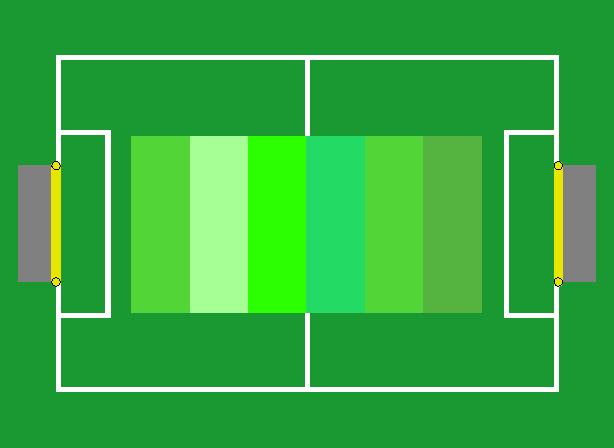
\includegraphics[width=0.6\columnwidth]{figures/walking-challenge}}
\caption{The field layout for the Walking Challenge: Six pieces of different carpets are placed next to each other between the two penalty areas. Each piece of carpet is about 1 meter wide and 3 meters long. A participating robot starts in the center of a penalty area, facing the goal on the opposite side of the field.}
\label{fig:walking_challenge}
\end{figure}

The carpets are arranged with increasing (expected) difficulty.

A robot can only receive one score per carpet. The order of mastered carpets does not matter. The order of performed actions does not matter, too. Therefore, it would be possible, for instance, to walk straight over all carpets (and gain 1 point for each carpet) and to return to some of the carpets afterwards to achieve higher scores on these carpets.

The carpets will be brought to the competition by TC members and the teams. On site, all available carpets will be presented and six carpets will be selected for the challenge. The selection should cover a broad range of (un)evenness and slippage. All carpets will be green (in any shade) but do not need to be uniform.



\newpage



% % % % % % % % % % % % % % % % % % % % % % % %



\section{Any Place Challenge}

Unlike humans, which are able to play soccer (at least at a basic level) independent of most environment features (\ie size and color of the ball, lighting, structure of the ground, size of goals, ...), most soccer robots still rely on very strict specifications of their environment. In recent years, the Standard Platform League addressed this issue by removing artificial field elements such as the border or additional beacons as well as by holding technical challenges that require playing under varying lighting conditions (2004) or playing with any ball (2009).

This challenge will be about shooting a (standard) ball into a (standard) goal that is not placed on an SPL field but on the floor of some room or hall at the RoboCup venue. The TC will determine the exact place but keep it secret to all participating teams. The chosen place will be challenging but reasonable, \ie, for instance, the ground will be even and hard and there will not be many orange features or yellow walls in the environment.

At the beginning of the challenge, everybody meets at the SPL area. The TC will fetch an official ball and one official goal. Every participating team will bring one robot. From then on, it will not be allowed to change the software or configuration of any robot. The group walks to the place that has been chosen for the challenge. The goal is placed and starting points for the robot and the ball as well as the field of play will be marked. All markers will be (almost) invisible to the robot. 

Now, the robot has 3 minutes to score as many goals as possible. If a goal is scored, the robot as well as the ball are put back to the starting points. If the ball is out of bounds, it will be put back on the starting point and the robot remains in place. If a robot seems to run away, it will be put back on its starting point but the ball will remain in place.


\newpage



% % % % % % % % % % % % % % % % % % % % % % % %



\section{Autonomous Refereeing Challenge}

Dietmar has to add a description here.

\newpage


% % % % % % % % % % % % % % % % % % % % % % % %



\section{Sound Recognition Challenge}

Dietmar has to add a description here.



\end{document}

